\newpage 
\section*{\huge Section 2}
\section{User Manual}
The application can be obtained either  a USB or by downloading it from GitHub.
\footnote{{\url:https://visualstudio.microsoft.com/vs//}}
The application can run on any Windows laptop it does not need any requirements. When the application is obtained, the user can click the setup.exe file and set up the application and follow the instructions below.

\subsection{Start Up}

When launching the application, you will be directed to the Start-Up page, which features a numbered layout of its components in the figure below, accompanied by a brief description for each corresponding number:

\begin{figure}[h!]
\centering
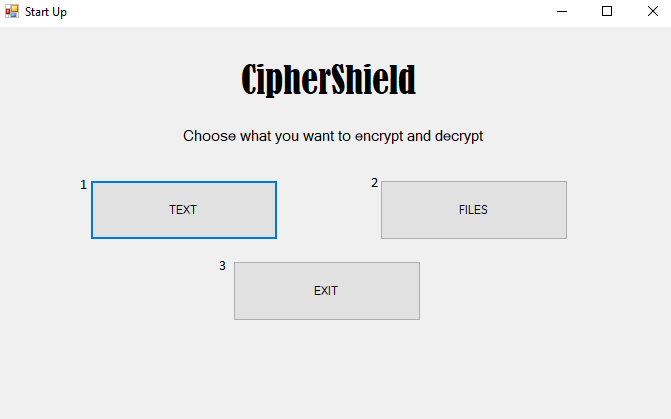
\includegraphics[scale=0.5]{Diagrams/StartU.png}
\caption{Start Up Page}
\label{fig:figure1}
\end{figure}

\begin{enumerate}
   \item This button will let you go to the Text Encryption Algorithms where you will encrypt and decrypt text.
   \item This button will direct you to the file encryption and decryption operations.
   \item Once you have finished using the application, simply click on this button to exit.
\end{enumerate}


\subsection{Text Encryption}
After clicking the Text you will be redirected to this Text Page which also has its own components:
\begin{figure}[h!]
\centering
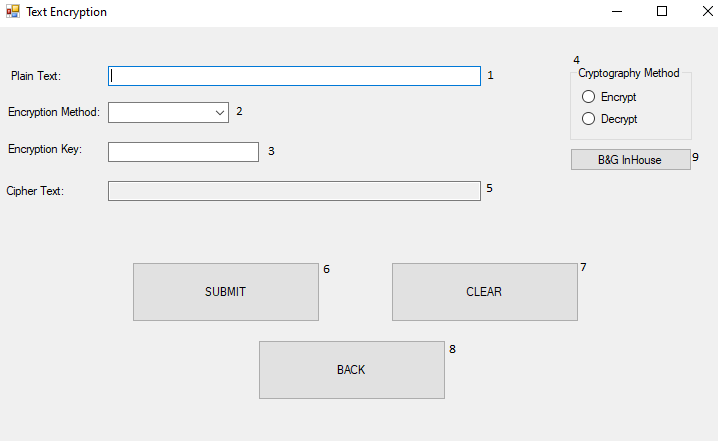
\includegraphics[scale=0.5]{Diagrams/TextEncryption.png}
\caption{Text Encryption Page}
\label{fig:figure1}
\end{figure}


\begin{enumerate}
   \item Textbox where you input the text you want to encrypt.
   \item Drop-down list for the different kinds of algorithms.
   \item Enter the key (note: keys differ with each algorithm).
   \item Radio buttons for encrypting or decrypting.
   \item After choosing numbers 1 - 4, press the submit button
   \item Output of the encrypted text.
   \item Clearing button to clear the textboxes, dropdown, and radio buttons.
   \item Back button to go back to the Start Up page.
   \item Going to the InHouse algorithm since it uses different operations than the other algorithms.
\end{enumerate}

\textbf{\\Instructions\\}
With regards to the text encryption methods: the user can input any message they want to encrypt and any key. \textbf{The Transposition and Vernam ciphers} only takes numbers as keys, and The \textbf{Vigenère cipher} takes letters only as encryption key. After putting in the key, you can choose any encryption method and choose to encrypt. When you want to decrypt make sure that the key is the same, if not it will not decrypt.

\subsubsection{B\&G InHouse}

After clicking the B\&G InHouse you will be redirected to this page which also has its own components:
\begin{figure}[h!]
\centering
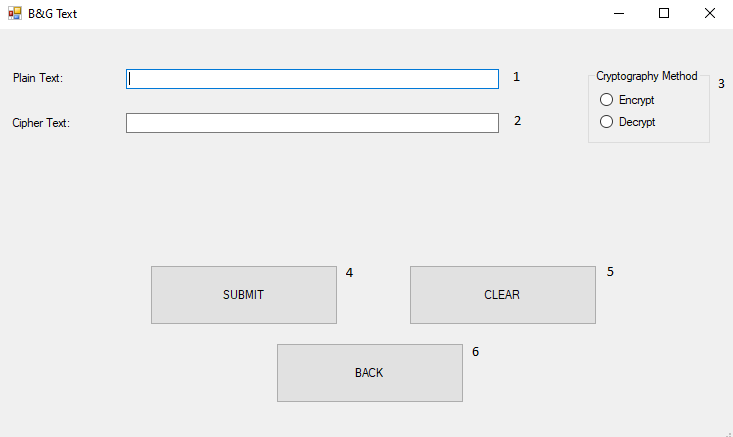
\includegraphics[scale=0.5]{Diagrams/custom.png}
\caption{B\&G Text Encryption Page}
\label{fig:figure1}
\end{figure}

\begin{enumerate}
   \item Textbox where you input the text you want to encrypt.
   \item Output of the encrypted text.
   \item Radio buttons for encrypting or decrypting.
   \item After choosing numbers 1 - 3, press the submit button
   \item Clearing button to clear the textboxes and radio buttons.
   \item Back button to go back to the Text Encryption page.

\end{enumerate}

\textbf{\\Instructions\\}
With B\&G InHouse, the user can simply enter the message they want to encrypt and choose a method. No key is needed.

\subsection{File Encryption}
After clicking the File button you will be redirected to this Text Page which also has its own components:

\begin{figure}[h!]
\centering
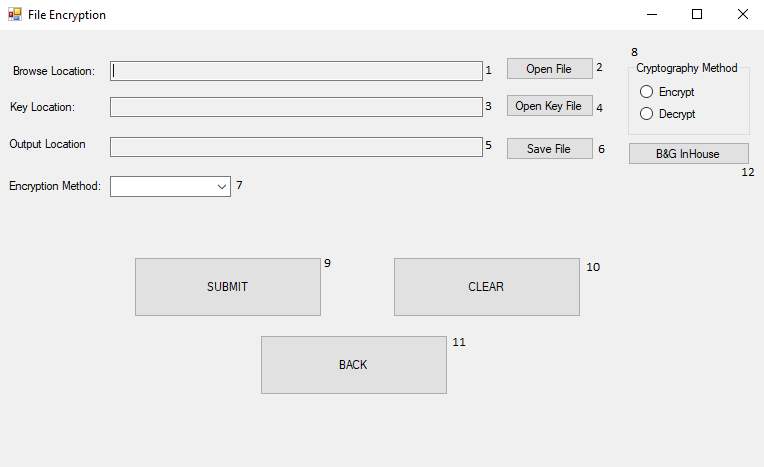
\includegraphics[scale=0.5]{Diagrams/FileEncryption.png}
\caption{File Encryption Page}
\label{fig:figure1}
\end{figure}

\begin{enumerate}
   \item Path of the file
   \item Button to locate the file you want to encrypt or decrypt.
   \item Path of the key file
   \item Button to locate the key file 
   \item Path of the output file
   \item Button to save the file 
   \item Drop-down list for the different encryption methods
   \item Radio buttons for encrypting or decrypting.
    \item After you are done, press the submit button
   \item Clearing button to clear the textboxes and radio buttons.
   \item Back button to go back to the File Encryption page.
   \item Button to go to the B\&G InHouse File Encryption.
\end{enumerate}

\textbf{\\Instructions\\}
With regards to the file encryption methods: the user can press the open file and choose any file they want to encrypt, the path of the file will be displayed, and the user will then choose a key file and  save the file that they want to encrypt. After that, they can choose any algorithm they want to use and choose to encrypt. When it is done a message will pop up. When you want to decrypt you select the decrypted file, in \textbf{Vernam cipher} you will select the key that is outputted and save the file, and press decrypt to get it to the original state. As well as the other algorithms.


\subsubsection{B\&G InHouse}
After clicking the B\&G InHouse you will be redirected to this page which also has its own components that will be discussed shortly.

To encrypt a file, you first select any file on your machine (such as docx, pdf, png, jpg, or any other file type), which will be displayed in the file path. Next, you enter a random key and choose to encrypt the file. Once you're done, press Submit and save the new file with any name you want. To decrypt the file, you follow the same steps but select the encrypted file instead.

\begin{enumerate}
   \item Path of the file
   \item Button to locate the file you want to encrypt or decrypt.
   \item The user does not need to input any key
   \item The user will generate any random key, the key for encrypting should be the same for encrypting
   \item Radio buttons for encrypting or decrypting.
   \item After you are done, press the submit button
   \item Clearing button to clear the textboxes and radio buttons.
   \item Back button to go back to the File Encryption page.
\end{enumerate}


\begin{figure}[h!]
\centering
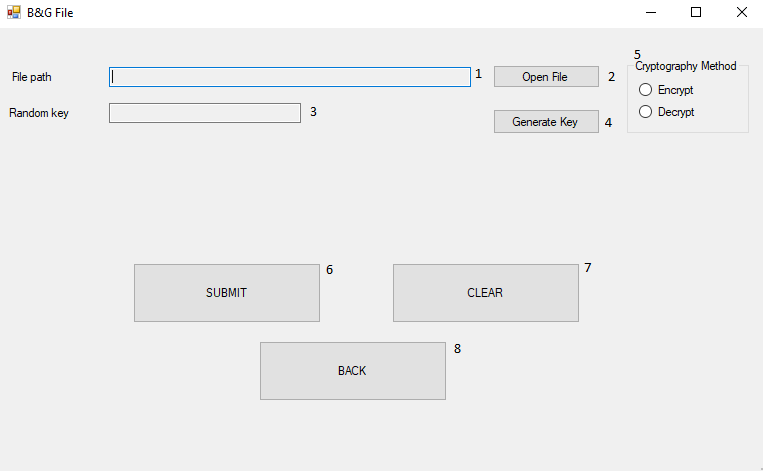
\includegraphics[scale=0.5]{Diagrams/customfil.png}
\caption{B\&G File Encryption Page}
\label{fig:figure1}
\end{figure}

\textbf{\\Instructions\\}
When you click Open File, you will go to any directory in your local machine, you select any file and click Open. The directory of the file will be shown in your File path on the application. Then you generate a random key, that will be used to encrypt and decrypt. It is a symmetrical key. You then click the Encrypt radio button and then Submit. It will lead you to the local directory where you have to name the new file. After naming it you will press save and the file will be encrypted. With encryption, you follow the same steps but you select the encrypted file and you select the decrypt radio button.
\\